% +==============================================================+
% |                                                              |
% |             Document created by Lennart Cockx				 |
% |                                                              |
% +==============================================================+

% +==============================================================+
% |                     Document settings				         |
% +==============================================================+

% Document formatting and includes
\documentclass[12pt]{article}
\usepackage[a4paper,left=3cm,right=2cm,top=2.5cm,bottom=2.5cm]{geometry}

%graphics for loading pictures into the document
\usepackage{graphicx}

%subcaptions for subfigures
\usepackage{subcaption}


\usepackage[hyphens]{url}
\usepackage{hyperref}
\usepackage[none]{hyphenat}
\providecommand{\keywords}[1]{\textbf{\textit{Index terms---}} #1}

\usepackage{multicol}

% Bibliography should use APA styliing
\usepackage{apalike}
\bibliographystyle{apalike}

% Change the gap size between the columns
\setlength{\columnsep}{15pt}

% This line adds a column separator between columns
%\setlength{\columnseprule}{0.1pt}


\usepackage[raggedright]{titlesec}

\usepackage{enumitem}
\setlist[itemize]{leftmargin=*}

\newenvironment{Figure}
	{\par\medskip\noindent\minipage{\linewidth}}
	{\endminipage\par\medskip}


% \begin{multicols}{2} % \end{multicols}


%opening
\title{Application development with\\ Microservice Architecture in Enterprise Java\\ A Spring Boot Case Study}
\author{Lennart Cockx\\Guangming Luo}

% +==============================================================+
% |                    End of document settings			         |
% +==============================================================+





\begin{document}

\maketitle
\newpage
\tableofcontents
\newpage

\begin{abstract}
\noindent In this report we will explore various Java technologies and analyse what features they offer. The focus of this project is to find which frameworks are most suitable for quick prototyping of a business application. Constraints and other requirements will be defined and are then applied to a specific case study. At the end of this project we should have an excellent understanding of the technologies involved to make a online cash register application that handles orders and payment in restaurants. [WIP]
% todo will be changed when the rest of the text is finished
\end{abstract}
\keywords{JavaEE, Spring framework, Cloud, Microservices}


%\noindent\hrulefill
\section{Master Thesis Objective}
\begin{multicols}{2}
\subsection{Proposal}
This master thesis is commissioned by Faros, a Cronos group company specialized in the development of Java web applications and primarily focused on designing Rich Internet Applications. Development within Faros is done with Vaadin, Spring, HTML5, ExtJS, JavaScript, JSP, JSF, NoSQL and more.\cite{farosProposal} This means that during this thesis, special attention is given to these technologies in regards to design choices. Naturally, comparisons with other possible frameworks will still be done and valid arguments will be set forward to confirm these decisions.
\\\\
The following case study was proposed by Faros: designing an online cash register that can be used in restaurants or at events. Existing cash register systems can be expensive. For smaller establishments or temporary events, this initial investment could be too high. The idea is to use existing devices from employees and customers to handle the ordering and payment process.
\\\\
This project is an opportunity for us to learn about the frameworks and technologies used for the development of rich, interactive web applications. Additionally, we want to explore the best methods to  build a web application from scratch. Some key aspects that we will look out for are: Documentation availability, speed of new project setup, customizability, integration with other frameworks and security features. When given the corresponding documentation, it should be possible to reproduce this application. During the design and development of this project we want to describe the problems we faced and how we solved them. This will give other students the option to learn from our mistakes and hopefully help them increase their understanding of Java EE concepts. 

\subsection{Concept}\label{sec:concept}
%TODO if possible, shorten this section
At the start of the project we discuss the key aspects of this project with our coaches at Faros. Based on the requirements provided by them, combined with our own interests and targets, we define the general field we will be working in and the features we should develop. See \textbf{section \ref{sec:constraints}} for the constraints defined together with Faros.
\\\\
After we have a good overview of the key aspects for this project, we can start searching for the appropriate technologies. The choices we make here are based on the aspects we think are needed for developing a web application meeting the aforementioned requirements. After doing this we should have a list of tools, systems, frameworks and libraries that could potentially be used during this project. See \textbf{section \ref{sec:javalandscape}} on the Java EE landscape. After defining the subject of our case study, this list can be shortened to technologies specifically applicable to this project.For certain frameworks it will be difficult to obtain a shorter list, as they might all comply with the requirements. In this case we will make a selection of items to keep the scope of the project realistic. Usually the most widely used frameworks will be selected. If a deviating set is chosen this will be elaborated on in the corresponding chapter. 
\\\\
The next step is to define the case study in more detail. The standard procedure for application development will be followed. Relevant documentation will be constructed including a use case analysis, feature description ( Nice-to-haves versus Must-haves ), navigational models, UML diagrams and market research. After this we can start working on getting familiar with the chosen enterprise Java frameworks. See \textbf{section \ref{sec:casestudy}} for the full case study. At this stage we will also try out the different technologies we selected to be able to better compare their advantages and disadvantages. See \textbf{section \ref{sec:comparison}} for a comparison of technologies.
\\\\
As soon as we are sufficiently proficient with our chosen tools, we will start implementing the case study and use the knowledge we obtained to build a functional prototype for a realistic use case scenario. During the project we might come to the conclusion that certain choices we made were suboptimal or simply do not allow further progression. In such cases, we will adjust our trajectory and change to the appropriate tools. Any time such a decision is made we will mention it in this report and provide the matching argumentation as to why we made the switch. Apart from the implementation, there will be a separate chapter to showcase the resulting application. See \textbf{sections \ref{sec:implementation} and \ref{sec:results}} for the implementation and results, respectively.
\subsection{Project Requirements}
\subsubsection{Constraints}\label{sec:constraints}
As this project is appointed by Faros, there are certain guidelines we will follow during this study. The primary constraint is the usage of \textbf{Java}. As Faros is a Java consultancy company, the technology stack we use should match what the employees there utilize. Within Java we are still free to choose what frameworks will be used. Another constraint is that we should not aim to create a perfectly working application with extensive styling and fail-safes, but rather focus more on experimenting with various different systems to get a better overview of the big picture and compare these systems with each other. There are also certain project-specific constraints that will be detailed in the case study.
\subsubsection{Design focus}
During this thesis we will develop a application based on a case study as mentioned in section \ref{sec:concept}. This case study is a device used for guiding development, but it is not the primary goal of this thesis. Instead, it is a way that allows us to explore the technologies used in application development on an enterprise level. In particular, we want to look at the \textbf{microservices architecture} and what advantages or disadvantages this has over more traditional web development. We will explore the microservices architecture in detail and research all related technologies and principles such as service discovery, routing, load balancing and security.

\end{multicols}

%\newpage
%\noindent\hrulefill
\section{Research and Methodology}
\begin{multicols}{2}
\subsection{Approach}
We will take a quantitative approach in this paper, exploring and comparing frameworks for each of the features required for this project. This includes: General frameworks providing a way to couple web resources to Java code. Persistence providers, SQL or noSQL databases to store customer information. Object relational mapping tools to generate mappings from existing data-stores. Security systems to allow authentication and authorization in a safe way. Front-end frameworks, providing styling options and client side scripting. Plus any technologies related to the microservices architecture. Everything related to the case study is detailed separately in \textbf{section \ref{sec:casestudy}}
\subsection{Java Enterprise Landscape}\label{sec:javalandscape}
We will not discuss every existing tool in the Java environment, but it might be interesting to have a look at the current state of Java EE in the professional world. We will use the numbers from a survey published by Zeroturnaround to do our analysis.\cite{JavaEELandscape73:online} This website has a blog for Java web developers and will display a certain bias towards this usergroup. For more general statistics please refer to Stackoverflow's developer survey. \cite{DeveloperSurvey95:online}
\\\\
Currently the majority of Java developers work on full-stack web applications (67\%), a smaller group works on back-end code only (18\%) with the rest of the developers divided into batch scripting, mobile apps, desktop applications, etc... This shows us that only in a fragment of the projects specialization is considered beneficial. Usually developers know and work with both front-end and back-end technologies. This is also what we will do during this project, implementing both the front-end and back-end of the application.
\\\\
So which front-end and back-end frameworks are used by developers? The most commonly used web framework is Spring MVC (43\%), followed closely by Spring Boot (29\%). Practically, this means that over 70 percent of respondents use the Spring framework. Spring Boot itself is not really a framework, but rather a streamlined entry point to the Spring ecosystem with a "Opinionated Defaults Configuration" approach. \cite{SpringBootAdvantages67:online}\cite{SpringBootIntro23:online} Other common web frameworks are JavaServer Faces (19\%), Vaadin (13\%) and Struts (7\%). Other frameworks exist but are too numerous to list. For this project we will limit ourselves to analysing the most popular frameworks. This should give us a good idea of the advantages that web frameworks offer, and how they compare. Spring Boot in particular looks promising as it provides autoconfiguration for many properties which will be advantageous for people new to the Java EE platform. It is also worth mentioning that 17 percent replied that they do not use any framework. It can be concluded that for certain projects using a framework is not worthwhile. % This could also be a point of discussion for our thesis
\\\\
When working with frameworks, developers will make use of build tools to avoid having to manually invoke the steps in the compilation process. The most popular build tools for Java are Apache Maven (68\%), Gradle (16\%) and Apache Ant(11\%). While using a different build tool won't directly affect the result of a project, it is important to make an appropriate choice from the start, as this build tool will be shared by all teammates in a project. 
\\\\
To deploy the application, an application server is needed. For production, Tomcat (42\%) is the primary choices for running Java web applications. The rest of the users are quite evenly distributed over the other application servers with the most popular being Jetty (12\%), Wildfly (10\%) and JBoss EAP (7\%). Developers have the choice of running their own application server and deploying their apps to it or making an application with an embedded server. For us, using an embedded server will get our project up and running faster. We will also run an external server to learn how this changes the development cycle. 
\\\\
While not directly related to specific technologies, the survey also asked participants to indicate whether they have adopted a microservices architecture. This is interesting for us to look into as this will be the focus of this project. It seems that microservices have become quite popular in recent year for a variety of reasons, like separation of concerns, natural modular structure and excellent for continuous delivery platforms. \cite{WhyMicroservices48:online} Although it differs from the usual approach we learned during our education, using this architecture in our application might provide valuable insights if we succeed.  
\\\\
Something that is not mentioned in the survey is security. Basic security is expected in any web application, but implementing a secure system is difficult. Java EE already provides the building block for securing a web application, but part of the design is still up to the developers themselves.\cite{JavaEESecurity29:online} Modern Java web frameworks go a step further however, giving developers a production ready security system out of the box. E.g. with Spring boot using Spring Security offers a system with built-in authentication and authorization. Safety and resilience are key factors that have to be taken into account when developing our application. The choice for security will largely depend on which framework we work with. 
\\\\
Another aspect not discussed in the survey is front-end frameworks. Commonly, the interface of a web application is designed using HTML, CSS and Javascript. On top of this CSS and javascript libraries like Bootstrap and JQuery can be used to speed up development by giving access to pre-made modules for frequently used interface elements. Front-end frameworks such as AngularJS and libraries like React can be used to speed up development even further. They offer tools and guidelines to make designing interactive interfaces efficient and fast. Although we will also discuss these frameworks in this paper, priority will be given to technologies related to the back-end.
\\\\
Finally, what types of databases are used to store information? The most used database are OracleDB (39\%), MySQL (38\%) and PostgreSQL (29\%). All three are relational databases. The most used NoSQL databases are MongoDB (15\%) and Redis (8\%). Note that these results are multiple choice, as some projects use multiple databases simultaneously. For the case study, the selection of database will depend on the type of data we want to store. Most of our experience is with relational databases, so trying out a NoSQL database will be valuable experience.
\\\\
Hopefully this section gave some insight into the technologies used in Enterprise Java Development and how we will approach them in our project. We want to try out various technologies and determine those most suitable for the use case and our development style. In the next section a more detailed explanation of the technologies will be given. During the exploration of these frameworks we will already create a prototype for the case study. This will give us a better idea which features would be beneficial for this specific project.


\subsection{Comparison of technologies}\label{sec:comparison}
Even before we specify the case study for our project we can already try out the different technologies discussed in the previous subsection and make a selection of those we deem appropriate for this master thesis. Any choices directly related to our specific case study will be discussed in section \ref{sec:casestudy}.

\subsubsection{IDE's and build tools}\label{sec:idebuild}
While the development environment and build tools are essential in application development. The choice itself is based on the preferences of the individual programmer. This project started out with the Netbeans environment and Maven for dependency management. When we started using Spring we tried out the Spring Tool Suite based on Eclipse, but we finally settled on IntelliJ IDEA and Gradle. IDEA offers many tools often needed during development such as a database editor, gradle/maven task execution, ORM modules, bitbucket plugin support, REST client for testing, superior auto-completion and built-in support for many frameworks. There are several other advantages to using IDEA, but these were the most determining factors causing us to switch environment. For the build tool, Maven is actually not inferior to Gradle. Both support the dependency injection that we need for this project. The primary reason we decided to try it out was curiosity. Gradle is currently the default build tool in Android development with android studio, and it is also utilized in Grails and Netflix OSS. When comparing them directly, Gradle seems to offer a much richer feature set. \cite{GradleVsMaven48:online} When using this build tool in the project, we came to the conclusion that these extra features were not really a necessity for our specific application. We did stick to Gradle in the end though, as the DSL syntax that it uses makes for a much more readable build file in comparison to the XML notation that Maven uses. We did stumble upon some issues while using Gradle. It also uses the Maven repositories for its dependencies, which means that if you want to add your own dependency to the local Maven repository, you will need to enable the maven-publish plugin within Gradle and add the relevant build code to bundle it correctly. Compare this to Maven, where executing the install task achieves the same result. In general, the choices we made for this section are based on our own preferences and experiences during the project.
\subsubsection{General framework}
The general framework will be the decisive element in the case study we develop. It will determine what modules we can use during development and what the general architecture looks like. Once we choose a certain framework, it will be difficult to convert to another. Our first iteration of this project started off as a plain Java EE project which served pages with the JSF framework. Apart from the configuration issues we had when first starting out, this worked quite well for simple servlets and beans. We created the necessary entity beans and business logic in an EJB package. Servlets, JSP files and static web content were packaged into a web archive. Both these packages were then combined into an Enterprise Application archive and deployed to a glassfish server. There were two big problems with this. First, configuring the application and server during the first setup takes a significant amount of time. The data sources must be configured in both the .ear as well as in the application server itself. When changing database or server this configuration must be redone. During development this can be a burden since we have to reconfigure should we want to make significant changes. Also, when we implement a microservices architecture, it will be necessary to repeat this configuration for every service. The other major problem is technology selection. Most technologies we use will be based on the specific requirements of the case study. For many other parts of the project there are still technologies that are used for any type of project, like what application server do we use?, what object mapping tool? and what security framework? plus many other systems that we didn't know the existed yet. Figuring out what systems we need and how to configure them will take a significant amount of time and they won't necessarily be the optimal choices. To avoid spending too much time here, we can use a framework which already implements these features for us in a production ready package. This way we can already start exploring and working with certain features without having to implement it all ourselves. Most frameworks still allow changing the preconfigured defaults to different system where necessary. Searching for these prerequisites led us to the Spring framework. Or rather, the Spring Boot ecosystem. 
\\\\
Like mentioned before, Spring Boot provides an opinionated toolset which gets you up and running in no time. All the necessary components are automatically configured and ready for deployment. For us this is ideal, we can quickly get started and we can learn about the necessary modules for deploying a Java Enterprise application by examining the code generated by the Spring Boot Initializer. Another interesting aspect about Spring is that it is considered an excellent base for designing applications following a microservices architecture. \cite{SpringMicroservices35:online} \cite{MicroservicesFrameworks85:online} Of course there are other frameworks that offer similar autoconfiguration and tools for implementing microservices, most notably Dropwizard and Vertx. The reason we decided to go for Spring Boot first is that, due to its popularity, it has great documentation and is very comprehensive, containing an extensive set of modules for all things required for modern web applications. Additionally, it is compatible with a wide range of other frameworks, so if we would need specific features from another framework this is still possible. This choice proved to be very good, we managed to reimplement the existing project we had in a matter of days and continued working in this framework. More details about our further steps in section \ref{sec:implementation}.
\subsubsection{Persistence providers}
%todo also need authorization
Data storage is practically utilized in any web application. We will need at least a way to store information for authentication purposes. In addition, we will likely need to store data related to the restaurant and menus. When storing relational data, a SQL database is typically used. Because we are taking a microservices approach and want to explore scalability, a NoSQL database might be more suitable.\cite{MongodbVsMySQL92:online} When handling diverse data types, improve scaling and modifying existing schemas, a NoSQL database can be beneficial. If we want to use this technology, it will take time to adjust. The principles behind designing NoSQL storage is completely different that relational data storage.
Since we are going for microservices, it is actually possible to use a different persistence provider depending on the service.
E.g. The default configuration for Spring Security makes use of a relational database. One table contains the usernames and passwords. This is connected with a one-to-many relationship to another table containing the role-user mapping, which in itself is connected to a table containing all the possible roles. This is a typical structure that would require a relational database. Using a NoSQL database is also possible, but requires a custom implementation of the UserDetailsService from Spring Security. On the other side we have to store order information from customers. Each order entry can hold an unstructured, arbitrary amount of items. It could also contain comments by the customer, but this field is not necessary. For this kind of data NoSQL might be more appropriate. If there are certain fields that we want to add or remove later on in development this also becomes much easier. Our final project can have a combination of MySQL and NoSQL providers, using the most suitable for each service separately.
\subsubsection{Object relational mapping tools}
ORM tools are useful utilities that offer automatic creation of Java entities from a database or vice-versa. It also makes an abstraction layer on top of SQL queries, which makes development much faster and prevents having to write SQL manually. Since it is likely that we will make use of NoSQL database in some of the services, an ORM is not useful anymore, since the traditional relational structure is not used in a system using NoSQL. The usage of ORM tools will hinge on the data structure we decide on.
\subsubsection{Security systems}
Security is something that is expected in a web application that stores information or provides functionality which should not be publicly accessible. In our case management of the restaurants and modifying the menus should only be permitted to employees of the corresponding restaurant. Account information, restaurant statistics and the order overview are all sensitive information and, again, should only be accessible by employees.
\\\\
Java EE provides various modules to secure a web application, but many of these modules still require quite a bit of configuration and certain features need to be implemented by the developers themselves. Things like encryption of passwords and https authentication might need to be created manually. Spring offers more extensive systems for securing a web application, available for use in any supporting framework. Spring security is a system that can be added to an existing project and enables a secure login and protection for specific pages and information with minimal configuration. The biggest hurdle that we will likely face is implementing these security features in a multiservices architecture. We will likely have to implement a separate service that handles security for all other services. In the case of Spring, this could be achieved by making an OAuth2 server.

\subsubsection{Front-end and Styling frameworks}
For styling our web application, we can make use of several Front-end frameworks and libraries. Usually the general web frameworks allow the serving of static web pages in the form of HTML and CSS pages. While making a beautiful interface is not the main focus of this project, we can still make use of a styling library such as Bootstrap or MDL to speed up and improve the design of our pages.
\\\\
Another trend in web development are responsive and reactive web pages. With the increase in mobile devices around the world, it cannot be assumed that people will visit a website on a large pc screen. Rather, most users will access web services from their phones or tablet devices. This means that when building a website we should try to make the interface scale properly for any size of device. Going even further than that, it is possible to improve performance by only reloading separate elements of the page and not redirecting to a new page each click. For this we will look at popular front-end modules like AngularJS and React. 
\subsubsection{Application architecture and microservices}



\end{multicols}
%\noindent\hrulefill
\section{Application Implementation}\label{sec:implementation}

\begin{multicols}{2}

\subsection{Case study summary}
In this project, a case study is used to define the functional requirements for development. During the implementation, we will keep these requirements in mind. The idea is to showcase a multiservices architecture using a relevant application prototype. Here is a small summary of what this case study entails: We will develop a web application to be used by restaurant owners or event organizers. They can apply for an account, giving them access to a public webpage where they can manage their establishment and employees. They can also create and modify menus for their restaurants or events. Customers coming to these places can use their mobile devices to access the corresponding menus and order food and drinks directly from their device. Employees assigned by the manager can see and process these orders from their own computers or mobile devices. We want to create an ecosystem for these purposes without needing specialized devices, with the necessary infrastructure running in the cloud. For a complete overview of the case study, see \textbf{section \ref{sec:casestudy}}.

\subsection{Development Process}
\noindent In this section, the actual process for the implementation of the project will be laid out. We will present a chronological progression of the project and discuss what we implemented and what roadblocks we encountered.
\\\\
As mentioned in section \ref{sec:idebuild}, we initially started out with a project made in Netbeans using Java EE serving JSP pages. This was a monolithic application that included client, business logic and database. This was our first experience with Enterprise java development. We had a locally hosted Payara server which we used to deploy our enterprise application archive. A simple SQL datastructure was running on an external MySQL server, which can been seen on figure \ref{fig:sqldiagram}
\begin{Figure}
	\centering
	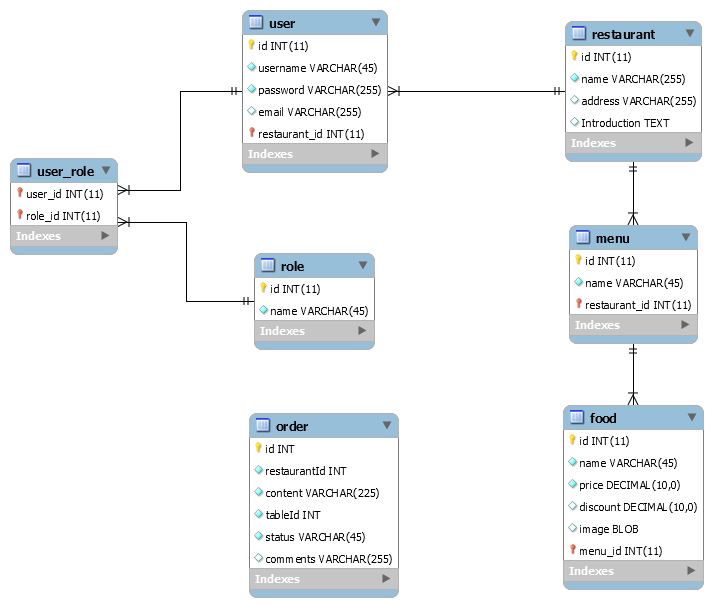
\includegraphics[width=\linewidth]{illustrations/database.png}
	\captionof{figure}{Original MySQL datastructure: This image shows the prototype relational model we used while working with a single SQL database}
	\label{fig:sqldiagram}
\end{Figure}
\noindent After our initial research we switched over to Spring Boot and recreated the original project. We still kept the previous database. The Payara server was replaced by the internal server that Spring Boot uses. This is a tomcat server that is packaged together with the resources and java code into a single executable .jar. This is great for testing as we just have to execute this one file to start our application server, deploy the project files to it and launch the server on the port we specified.
\\\\
For this application we used hibernate to generate Java entities from the database model we designed. There was also a basic version of Spring security running in this project that only allowed access to certain pages based on the role assigned to the account you logged in with. When logged in, users could access the restaurant page they were assigned to. At this time the page was a blank template on which the corresponding restaurant's name was shown. From the start we chose to split up the functionality of the program into different modules, we hoped that this would enable us to more easily divide the project when changing to a microservices architecture.
\\\\
Now that we have a functional Spring Boot application, we can start adding the services we need for our case study. The final application should have the following services:

\begin{itemize}
	\raggedright
	\item \textbf{Restaurant service}\\Provides the name, address and a description of each restaurant registered with our webapplication.
	\item \textbf{Menu service}\\Holds the menu categories for a specific restaurant.
	\item \textbf{Food service}\\Has a list of food items associated with a category and registers their price.
	\item \textbf{User service}\\Manages everything related to the login and authorization of employees and managers.
	\item \textbf{Order service}\\Takes and stores orders made by customers.
\end{itemize} 
Implementing these services went smoothly as we can avoid writing a lot of boilerplate code by using the autoconfiguration from Spring Boot. When creating the various services, they are configured with the \textit{@Service} annotation. Functionally this annotation works the same as \textit{@Component}, and allows this class to be used with automatic bean detection on the application classpath. When used, these classes will be instantiated as a singleton beans. The primary reason the \textit{@Service} annotation is used instead is to indicate what type of component we are creating as defined in Domain-driven design.\cite{ComponentAnnotationDifferences34:online}\cite{ServiceAnnotationSpring48:online} We purposefully make a distinction between presentation, service and data access modules to make classification easier.
\\\\
Currently, the services use entities to access relevant data from one MySQL database. The process used to generate these entities is as follows: First, a UML diagram was created including all tables and relations required, seen on figure \ref{fig:sqldiagram}. This diagram was then forward-engineered into a local database and filled manually with sample data. Then, the Hibernate provider for Java EE persistence was used to generate Java entities based on this database. This gives us entities which can be retrieved and persisted on the SQL server. To do queries on the database, e.g. to search for users or restaurants, we would have to write our own queries. Luckily Spring Data gives us a \textit{JpaRepository} class that we can extend to generate the queries automatically. By extending this class, we immediately have access to all basic operations to create, modify and remove entries from the database. A simplified notation can be used to create the necessary queries. For example, we need a way to find restaurants based on ID or name. The only thing we have to do is create a class that extends \textit{JpaRepository} and declare 2 methods: \textit{Restaurant findRestaurantByID(int id);} and \textit{Restaurant findRestaurantByName(String name);}. Spring Data will configure the rest.
\\\\
Once we specified these services with the correct annotation, they can be used in the business logic. Using \textit{@Autowired} allows us to refer to a registered component or service. At this stage the services are utilized from within the controllers that we use to map the webpages served by our application. \textit{@RequestMapping} is used to map certain addresses to their corresponding HTML pages. These pages are parsed with the Thymeleaf templating engine to include the data we receive from the services. At the start we only used Thymeleaf to pass database information to the web pages. We soon had multiple pages, often with duplicate code. This made us look into Thymeleaf fragments. All commonly used interface elements were added on a general file, where the content was filled in with fragments depending on the purpose of that page. A good example of this is the navigation bar, which should be visible on every page.
\\\\
At this point we have a functional web application that has pages to display restaurant information from the database. These pages are protected by a basic Spring Security system. Users can only access the restaurant they are assigned to. An administrator account can create new users and bind them to a specific restaurant. To limit the amount of similar pages, we wanted to show or hide certain parts of a page depending on the authorization of the current user. While this is easily implemented by using the controller model parsing from Spring MVC, this would require us to pass security configuration in all the methods of each controller. A more streamlined solution would be preferable. This lead us to the Spring Security dialect for Thymeleaf. Including this dependency allows the usage of Spring security entities directly in the HTML code, which prevents a significant amount of redundancy in the controllers. This can be used, for example, to show the name and privileges of the logged in user.
\\\\
When certain errors occur during authentication or on our pages in general, it can be useful to have an error page to display what went wrong. We used the Spring Boot Actuator package to create a default error page. This page does not use any styling and has a limited amount of information, so we implemented a custom \textit{ErrorController} that can show stack trace information and matches the design of our other pages. During this time we finished much of the business logic and static pages for the case study. However, It was still a monolithic application running on a single SQL server. The next step would be to start creating REST controllers to enable REST requests to the services. This is needed to build a REST API, allowing access to the services after splitting them up in separate modules.
\\\\
Changing the output of a controller to is relatively straightforward. We make new controllers for each service using a \textit{@RestController} annotation instead of \textit{@Controller}. Instead of returning String templates, the mappings should be changed to return the entity classes. In practice this will return a JSON object to the client doing a REST call. Having these REST controllers allows for effortless communication between the various services and the application server. Now we are in a good position to start separating the services into different modules. The result of this separation is shown in figure \ref{fig:microservicessplit}.
\begin{Figure}
	\centering
	
\includegraphics[width=0.9\linewidth]{illustrations/placeholder.jpg}
	\captionof{figure}{Project structure after splitting into separate modules: Instead of the single monolithic application, the project now has a separate module for each service. Each module consists of an REST access point, a service that handles the REST calls and an individual database. This database can use SQL or NoSQL depending on the data it contains.}
	\label{fig:microservicessplit}
\end{Figure}
\noindent Splitting the existing project into modules that can run and function proved to be quite a difficult task. One of the major problems was the database structure. It is possible to have all services connect to one central database, but this conflicts with the microservices concept. There would still be a central point of failure and scaling would still be limited to replicating the database on multiple servers or using application specific sharding. Instead of that we created separate databases for each service. We had to rethink the way we approached our data, as direct relations are not possible any more. Another disadvantage is that the initial migration from a monolithic application takes a significant amount of time. For us it took around one week to translate the single large project into a functioning microservices system. After getting the first few services to work, this process does speed up. Because the services are simplified to their most basic form, implementing additional services after the first one is only a change in the business logic. During migration, we also noticed that certain existing systems break when moving to a microservice ecosystem, Spring security in particular. Instead of using the default configuration, an additional services that provides security for all services is required. Similarly, many of the technologies which are easily used in a monolithic application become much more difficult it is split into individually functioning parts. We have to take into account that these services are running on different ports and could be running on completely independent servers.
\\\\
Although there were several issues changing over to microservices, it did also bring noticeable advantages for development. The different services now have a REST API that returns a JSON object instead of Java entities. This is very convenient when making additional clients for accessing our application. We can do a http \textit{GET} or \textit{POST} to the corresponding services and we will get JSON back that can be immediately used to access the necessary information. We used this to create a native android application to be used by employees at a restaurant. More detail about this here: % put a reference here
Another interesting aspect of this structure is that we can build modular web pages that get their information from multiple services. If a certain service is down or is experiencing connection problems the page can still be loaded. The missing content is simply not shown and we show a message on screen to indicate that a certain service is having issues. Thanks to the microservices architecture, only basic exception handling is needed to implement this.
\\\\
We are now at the point where we have a functional application build upon a microservices foundation, but there are still some practical issues with the current structure. Currently, there is one instance of each service running in their own container, each bound to a specific port number. To access an API, the address and port of the service have to be known. For the application server accessed by browser clients these adresses can be hard-coded, although this is not recommended.(See the next paragraph about discovery.) For other clients this is more difficult, they do not know which addresses they can use the access the APIs. Hard-coding this would be detrimental as it would require an update of the application each time infrastructure changes are done. For example when changing the host of a certain service. The solution we used was creating an extra service that functions as a gateway for all the API endpoints. The Spring cloud dependency offers the foundation for this gateway under the form of Zuul, developed by Netflix. \cite{NetflixZuul76:online} Implementing this gateway allows us to accept requests that include the service name and route these requests to the corresponding service by specifying their addresses in the Zuul gateway configuration. The API gateway functions as a reverse proxy, illustrated in figure \ref{fig:apigateway}. The services are now accessible from the android application without the need for specific addresses or ports.
\\\\
\textbf{Service Discovery}\label{sub:discovery}\\
While we have a functional Api gateway system now, we are not yet making use of all the advantages the microservice architecture offers. For example, if we want to run multiple instances of the same service for redundancy or load balancing, how do we determine the addresses of these services? We cannot simply add more routes to the Zuul gateway, this is not scalable. Instead we created yet another service that works with the Eureka system, also part of the Netflix open source software. Eureka provides a discovery service on which other services can register themselves. The Eureka server holds a list of each services registered to it, as well as the amount of instances available and on what addresses they are located. To have a service register itself to this discovery server they have to be instantiated as an Eureka client. On startup they will connect to the server and register themselves with the corresponding information. This opens up a lot of possibilities, we can know host each service multiple times and if one instance crashes or has connection issues the application will still function. Eureka also does basic round-robin load balancing, which means that incoming api calls from clients will be spread over the pool of available services, which helps with performance.
\\\\
With the inclusion of a discovery service and Api gateway we now have a fully functional system that makes use of the advantages a microservices architecture brings to web development. 




% todo more information about http benchmarking
%todo add issues: 
%todo biggest parts: Security, Spring MVC, Thymeleaf, microservices, discovery, gateway.

\end{multicols}
%\newpage
\section{Case study: Online cash register}\label{sec:casestudy}
\begin{multicols}{2}
\subsection{Introduction}
The goal of this case study is to create a service that can be used at events and in restaurants to process orders made by customers, relay these orders to the waiters and chefs and handle the payment. This service should include an application that clients can use to view the menu and order items from it. Waiters also have their own application that can place and acknowledge orders. These orders will be send to a central system that manages all the required information. See fig. \ref{fig:usecase} for a use case diagram.
\subsection{Existing systems}
%TODO More detail needs to be added. also move this to research and methods
Before creating our own Online cash register application we searched for similar systems that already exist. One of such systems is Gloriafood \cite{Gloriafood:online}. This is an online system that allows any restaurant owner to sign up and start receiving orders online. A extensive layout is available where you can add a menu and payment options.
\\\\
Similarly, there is ChowNow \cite{Chownow:online}. This service also handles online ordering and payment with no extra input required from the restaurant manager. ChowNow will also create a custom branded mobile application to showcase the brand and food of the restaurant.
\\\\
Both of these systems are focused on the online ordering aspect and not so much on allowing people to use their devices to order food on location. In this project we want to put the emphasis on the latter part, creating an application that is meant to be used at the location itself.
\subsection{Use Cases}
In this case study we can identify several distinct actors that will interact differently with the application.
\paragraph{Customer}
The customer is the primary user of this application. They access the menu of a specified restaurant or event. They can place orders, either via the application itself or from a waiter with their own device. Finally, they can pay for the orders that they placed. Again, either via the application or a waiter.
\paragraph{Waiter}
Like the customers, the waiter can access the menu of their restaurant and place orders for their clients. In addition to this they can display an overview of the currently queued orders, with the corresponding table numbers or location. They will also handle payments from customers through the application, or accept payment in other forms of currency.
\paragraph{Chef}
The chef can access similar functions as the waiter. Additionally, they can modify the status of an order and mark it as completed or in progress.
\paragraph{Manager}
The manager can modify the menu and change prices. They can also create accounts for employees and give them the corresponding privileges.\\

%should also have some information about multi-tenancy
\begin{Figure}
	\centering
	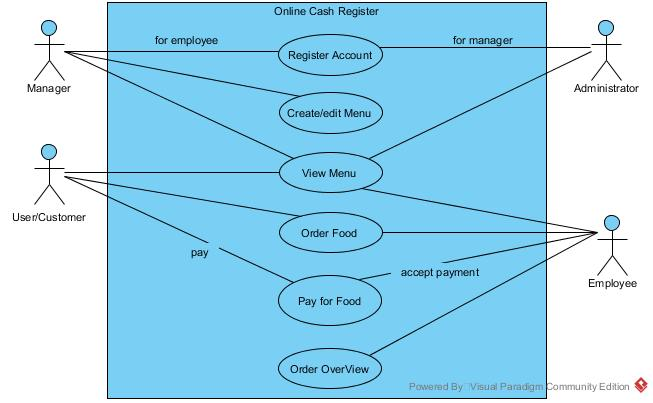
\includegraphics[width=\linewidth]{illustrations/usecase.jpg}
	\captionof{figure}{Use Case Diagram}
	\label{fig:usecase}
\end{Figure}

\subsection{Must-haves and nice-to haves}
As soon as we had the use cases defined, we can specify what features are absolutely essential and which are optional. This was done in collaboration with our coaches at Faros and gave us the following specifications.
\paragraph{Must-Haves}
\begin{itemize}
	\raggedright
	\item The system can be used by multiple managers or event-organizers simultaneously. 
	(\textit{Multi-tenancy})
	\item A central application will handle orders and payment. 
	(\textit{Central application})
	\item Waiters can use an application to send the orders of customers to the kitchen and accept payment. 
	(\textit{Employee interface + Payment system})
	\item Customers can view the menu of the restaurant/event with their mobile device. 
	(\textit{Customer interface})
	\item An order overview is available for the waiters and chefs. It shows the completed orders and orders which have to be made. 
	(\textit{Order overview})
	\item Customers can add comments to certain orders. E.g. no tomato
	(\textit{Special requests}) 
	\item Customers can place their own orders with their mobile device. 
	(\textit{Customer Mobile ordering})
	\item Prevent customers from making ridiculous orders or misusing the system.
	(\textit{Misuse prevention})
\end{itemize}
\paragraph{Nice-to-Haves}
\begin{itemize}
	\raggedright
	\item Event organizers can run the central application on their own local network. 
	(\textit{Local network hosting})
	\item After an order is finished, the completed order number is shown on a big screen. 
	(\textit{Take-a-number/Now serving System})
	\item The manager can find statistics on his restaurant and orders via a web app. 
	(\textit{Order Statistic}s)
	\item Customers can split the bill or combine orders 
	(\textit{Bill splitting})
	\item Provide an easy way for customers to use our system at an event/restaurant. Even if they don’t know it yet. 
	(\textit{Easy access})
	\item Customers can order additional food or drinks. This will be added to the total bill.
	(\textit{Multiple orders})
\end{itemize}

\subsection{Design Choices}
\subsubsection{Client}
%Possibly insert pictures we designed
%This part will need to be reviewed as changes to the design were made
We want to make an application for customers of restaurants and events. The customer can use this application to get an overview of the available menu items and prices. If the customers have decided, they can order the desired dishes straight from the application. Finally, the customers can pay for their meal with this application.
We can differentiate a couple of different scenarios when the customer goes to a restaurant or event that supports this system. We assume that a web app is used. If a native or hybrid application is used, installing the app will be an additional step before using the system.
\\\\
After (or before) the meal is finished, customers should be able to pay directly from within the application or pay a waiter. When using the application to place an order for multiple people, the customers should have the option to order and pay separately or order together and split the cost. 
For example: Three people want to place an order, two of which have access to the application. 
\begin{itemize}
	\raggedright
	\item One person can place the order for the entire group.
	\item One person can order for himself and the person without the application. While the third person makes his own choice with his own device.
	\item The two persons with the application order for themselves, while the other person orders something from a waiter.
\end{itemize}

\noindent 
In all three cases the order will be combined into one order for that table. After the meal the bill can be paid for.

\begin{itemize}
	\raggedright
	\item One person decides to pay for the entire bill. This can be paid to a waiter or with his application.
	\item Each person pays for the part he ordered separately, with the price corresponding to what they ordered.
	\item Everyone decides to split up the bill equally, dividing the total cost over three people. 
\end{itemize}

\noindent
Typically, when people eat at a restaurant, they will place multiple orders. During the meal additional drinks might be ordered and at the end of the meal some people might want a dessert or coffee. We must design the application so it can accept multiple orders and display the sum of these orders at the end of the meal.


\subsubsection{Employee}
To be able to interact with customers using this system, the waiters and chefs will need their own version of this application. They will need to get an overview of the current orders placed and they should be able to modify and confirm these orders.
\\\\
The order overview will have all the relevant information of the order: The different dishes and drinks ordered by the customer, the table from which the order was placed, the price and the status of the order. Additional information such as a time and date and an order number can be added for statistical purposes.
The order overview could look something like displayed in fig. \ref{fig:orderview}.
\begin{Figure}
	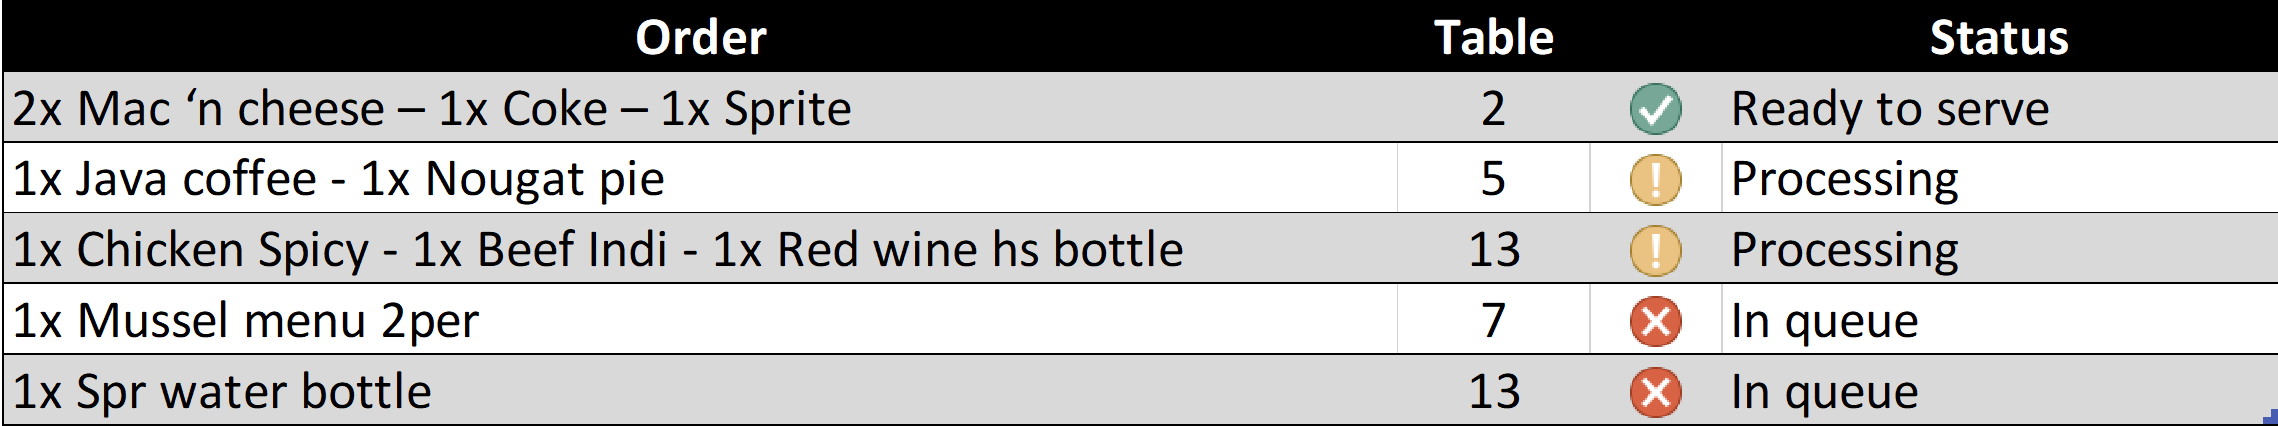
\includegraphics[width=\linewidth]{illustrations/orderview.PNG}
	\captionof{figure}{Example Order Overview}
	\label{fig:orderview}
\end{Figure}
Whenever an order is served, it will be removed from the overview and the next item will be moved up. When the bill is requested, all orders from the corresponding table will be added together. After payment the orders for that table are reset to allow the next customers to place their order.
\\\\
In some cases, an order might be wrong or a mistake with the number of dishes is made. The application should be flexible and allow a waiter to make small modifications to the order to correct a mistake.
Additionally, a customer might make a special request for his order. This can be due to allergies or plainly because of a certain preference. It might be useful to provide a bit of space to the order overview for extra remarks.
\\\\
An order might contain a lot of different items. The full names of these items will take a lot of space in the order overview. Typically, a shorthand notation is used by waiters to more efficiently note down and read orders. A similar system could be used for the order overview.
Also, for showing the menu to the customer we will display a vertical list with the name of every menu item. This list will contain detailed information like the name of the dish, the ingredients, pricing and possibly even a picture. These menu items can be sorted into categories for easy navigation. On the other side, the waiter does not need all the detailed information. Instead a compact and efficient layout is preferred to be able to easily take an order. This could be a grid layout with simple icons or abbreviations for each dish. See fig. \ref{fig:waitercustomer}.
\begin{Figure}
		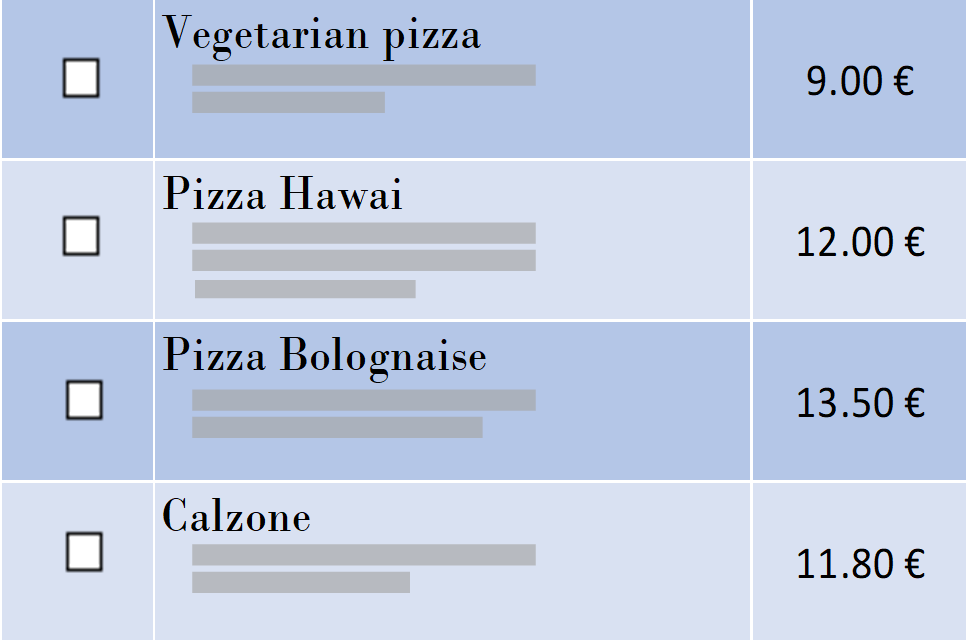
\includegraphics[width=\linewidth]{illustrations/customermenu.PNG}
		\captionof{figure}{Customer Menu Layout}
		\label{fig:menucustomer}
\end{Figure}
\begin{Figure}
	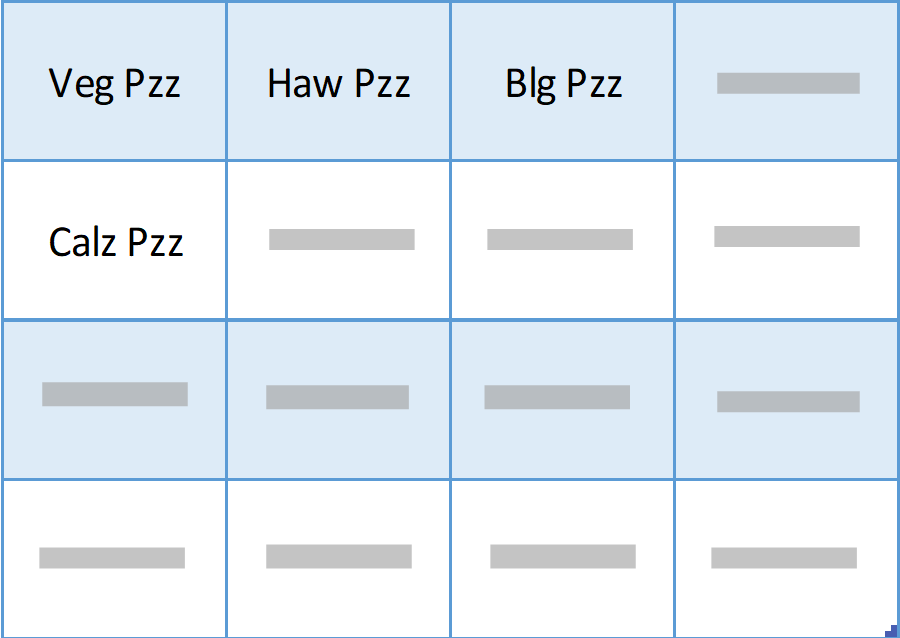
\includegraphics[width=\linewidth]{illustrations/waitermenu.PNG}
	\captionof{figure}{Waiter Menu Layout}
	\label{fig:waitercustomer}
\end{Figure}
\noindent \\It is possible that certain people with bad intent might try to place orders for ridiculous amounts of food, repeatedly place small orders to fill the system or even place orders for another table. Some of these situations can be prevented with proper programming, e.g. limiting the amount of orders one table can make each minute. Another way to prevent some of these issues is to have waiters confirm orders on their device before adding them to the kitchen. In day to day use, these scenarios will be rare, but it’s still important to think about the possible problems that might occur. While a user account for the customer might be desirable to track certain statistics and prevent misuse of the system (like mentioned above), requiring an account might not be interesting, as this can make the process of using the application slow and unintuitive for the customer.


\subsubsection{Manager}
The manager will be able to create new accounts for employees that work in their restaurant. They can modify properties of the restaurant and alter the menu and prices. 
\\\\
One of the most important aspects to consider here is multi-tenancy. The application should not only provide an interface for a certain restaurant but should be usable by different managers who own different restaurants. In other words the application should be generic and allow for customization for each restaurant separately.
%\subsubsection{Remarks and challenges}
%\subsection{Major issues and their solutions}

\section{Results}\label{sec:results}
In this section, an overview of the final application prototype will be given, along with possible improvements that can be done in the future.
\subsection{Final Prototype}
The final version of our application is divided into several modules which can be seen on figure \ref{fig:applicationdiagram}

\begin{Figure}
	
\includegraphics[width=\linewidth]{illustrations/placeholder.jpg}
	\captionof{figure}{Application diagram}
	\label{fig:applicationdiagram}
\end{Figure}

The application can be accessed via a browser client on any device or employees can use our native application on android devices. When using a browser, the user will connect with an application server that serves html pages. Customers will be greeted by a menu page of the restaurant they browsed to. From this page they can make a selection of items and place an order. These features do not require the user to be logged in. Employees and managers can log in to access more functionality. Once logged in, employees can view an overview of the currently placed orders and update their status. They can also modify the menu, creating new menu items or removing them. They can do this only for the restaurant they are assigned to. Managers will have the rights to create and manage employee accounts.

\subsection{Possible Improvements}

\section{Conclusion}


\end{multicols}

\newpage
\section{References}

\bibliography{document}


\newpage
\section{Appendix}
\subsection{List of technologies used}
Underneath, a list of technologies used during this project can be found. Technologies present in the final application will be indicated in \textbf{bold}.
\begin{itemize}[leftmargin=20pt]
	\item \textbf{Java + Java EE}
	\item \textbf{Spring Boot} - Bootstrapper used on top of Spring MVC
	\begin{itemize}[leftmargin=20pt]
		\item \textbf{Spring MVC} - Java web development framework
		\item \textbf{Spring Security} - Java web security dependency
		\item \textbf{Thymeleaf} - Templating engine for web pages.
		\begin{itemize}[leftmargin=20pt]
				\item  \textbf{Thymeleaf Security Dialect} - integration module for Spring Security
		\end{itemize}
		\item \textbf{Spring Actuator} - Application endpoints for monitoring and management
		\item \textbf{Spring Data} - Persistence APIs for database access
		\begin{itemize}
			\item \textbf{Spring Data JPA} - Persistence API for database access and Object mapping
			\item \textbf{Spring Data MongoDB} - Persistence API for NoSQL database access
		\end{itemize}
		\item \textbf{Spring Devtools} - Spring-specific tools useful during development. E.g. Hotswapping, auto-disable template caching and automatic restarts
		\item \textbf{Spring Cloud} - Provides tools and patterns that assist in building distributed applications
		\begin{itemize}
			\item \textbf{Netflix Zuul} - Reverse proxy implementation for Api gateway pattern.
			\item \textbf{Netflix Eureka} - Discovery server and clients for managing and load balancing services
		\end{itemize}
	\end{itemize}
	\item \textit{Web Development}
	\begin{itemize}
		\item \textbf{HTML} - Markup language used for web pages
		\item \textbf{CSS} - Markup language for web pages styling
		\item \textbf{JavaScript} - Scripting language to make web pages dynamic
		\item \textbf{jQuery} - Javascript library to simplify and extend JS development
		\item \textbf{Material Design Lite} - CSS and Javascript library for designing web pages using material design
		\item \textit{React} - A component-based Javascript library for building UIs
		\item \textit{AngularJS} - Structural framework for building dynamic web applications
		
	\end{itemize}

	\item \textit{Mobile Development}
	\begin{itemize}
		\item \textbf{Android SDK} - Software development kit for android apps
		\item \textit{PhoneGap} - Multi-platform Mobile application development framework
	\end{itemize}
	\item \textit{Development Tools}
	\begin{itemize}
		\item \textbf{Intellij IDEA} - Integrated development environment for the Java virtual machine.
		\item \textbf{Gradle} - Build automation system
		\item \textbf{Maven} - Build automation system
		\item \textbf{MongoDB CLI} - Command line interface for managing MongoDB 
		\item \textbf{MySQL workbench} - Tool for managing MySQL database
		\item \textbf{Android Studio} - IDE for native android development
		\item \textbf{Git} - Version control system
	\end{itemize}
	
	
	
	 
\end{itemize}
\subsection{Problems and their solutions}
\subsubsection{Problems with database model foreign keys}
\begin{itemize}
	\item When a foreign key is also included as part of primary key, you cannot remove this foreign key or drop the primary key.
	\item Remove the schema and regenerate all tables; if not necessary, do not include foreign keys as part of primary key.
	\item You cannot remove a table when one of the columns is used as foreign keys in other tables. Similarly, you cannot truncate a table when foreign keys in other tables have been instantiated.
	\item When instantiating an entity with a foreign key, errors usually appear when the foreign key doesn't have a valid value or empty.
\end{itemize}

\subsubsection{Thymeleaf-related issues}
\begin{itemize}
	\item You cannot give two th:each properties in one div, which means you cannot loop through two lists at the same time.
	\item You can use Thymeleaf to check if the user is authenticated by adding \textit{sec:authorize = "isAuthenticated()"} to a div, and the div will not show up if it’s false. Same for \textit{sec:authorize = "hasAuthority('ADMIN')"}, the div will only show up when the user has authority of admin. E.g. \textit{<a sec:authorize = "isAuthenticated()" th:href = "@{/restaurant/name/}" class="mdl-navigation  link" href="">Restaurant</a>} (line 50 of navbar.html)
	\item If you want use model attributes from controller in JavaScript, th:inline = "javascript" has to be added to the script tag and use special format to use the attributes: \textit{var url = /*[[\${url}]]*/'url';} (see line 33-41 of account.html)
\end{itemize}

\subsubsection{HttpRequest POST problems}
\begin{itemize}
	\item Everything get post to the controller via HTTP is String, it’s up to the server to decide which type you want to decode. If you specify @Valid int tableId, the controller will try to decode the value to int and will introduce an error if it fails.
	\item Hidden input can be used to submit action where there is no input field. You can also put a hidden input field to normal form.
	\item RedirectAttributes can be used to pass data from post function after redirecting. This is specifically for Spring Framework. After initializing, you can use it like this: \textit{redir.addFlashAttribute("message"," This username is already registered!");} and in the redirected GET method, you can get the information by specifying \\\textit{@ModelAttribute("message")} final String message.
	\begin{itemize}
		\item Those flash attributes are passed via the session 
		\item They will be destroyed immediately after being used
		\item They are not visible in URL
		\item You are not restricted to String, but may pass arbitrary objects.
	\end{itemize}
\end{itemize}
\subsubsection{Appending URLs}
If you want to go to another base on the current page, you need add an "/"after.
e.g. current url:"www.mybase.com/home/" \textit{href="edit"} will lead you to "www.mybase.com /home/edit". If you current url is "www.mybase.com/home" \textit{href="edit"} will lead you to “www.mybase.com/edit”.

\subsubsection{Spring Security role checking on the server side}
You may check if the logged in user has a role of admin in controller final:
\textit{Authentication auth = SecurityContextHolder .getContext().getAuthentication();
SimpleGrantedAuthority AUTHORITY\_ADMIN = new SimpleGrantedAuthority("ADMIN"); org.springframework. security.core.userdetails.User user = auth.getPrincipal(); if(user.getAuthorities().contains (AUTHORITY\_ADMIN))\{
	model.addAttribute("isAdmin",true);
\}}

\subsubsection{Database issues}
"table","order" and other similar keywords cannot be used as table name or column name, SQL will fail.

\subsubsection{Creating a custom Maven/Gradle dependency}
Initially, we want to make a jar file and include it in our project, but we failed to use/refer to it. Later, we choose to create a local maven dependency, and compile it in the gradle dependencies.
How to make a maven dependency with your models?
Create a maven project with groupId = com.xxx and Artificial Id, under java folder, create pakage: com.xxx.models, put all your java files under that folder. Then do maven build.

\subsubsection{Combining microservices and Spring Security}
According to the tutorial from spring.io/blog, the author disable component scan in the main application and create all beans inside main.
However, this may cause an issue, because it will also disable the security configuration which is usually a separate config class. In this case, the whole project will use default spring security configuration (all pages need login).








\end{document}
